\documentclass[11pt,a4paper]{article}
\usepackage[margin=23mm,headheight=15pt,footskip=12mm]{geometry}
\usepackage{fontspec}
\setmainfont{NotoSansCJKkr-Regular.otf}[Path=fonts/,BoldFont=NotoSansCJKkr-Bold.otf,ItalicFont=NotoSansCJKkr-Regular.otf,ItalicFeatures={FakeSlant=0.12}]
\setmonofont{DejaVuSansMono.ttf}[Path=fonts/,Scale=0.8]
\XeTeXlinebreaklocale "ko"
\XeTeXlinebreakskip=0pt plus 0.1em
\usepackage{amsmath,amssymb,mathtools,graphicx,booktabs,longtable,array}
\usepackage[dvipsnames]{xcolor}
\usepackage{enumitem,fancyhdr,titlesec}
\usepackage[unicode,colorlinks=true,linkcolor=MidnightBlue,citecolor=MidnightBlue,urlcolor=MidnightBlue,breaklinks=true]{hyperref}
\hypersetup{pdftitle={BASS CR 다음 연구 루프: 실제 전자 주입원과 유한 나이 열 응답의 연결},pdfauthor={BASS CR research}}
\setlength{\parindent}{0pt}
\setlength{\parskip}{0.5em}
\setlength{\emergencystretch}{3em}
\setlength{\tabcolsep}{4pt}
\renewcommand{\arraystretch}{1.18}
\newcolumntype{P}[1]{>{\raggedright\arraybackslash}p{#1}}
\renewcommand{\contentsname}{목차}
\renewcommand{\figurename}{그림}
\renewcommand{\tablename}{표}
\renewcommand{\refname}{근거 자료}
\titleformat{\section}{\large\bfseries\color{MidnightBlue}}{\thesection}{0.7em}{}
\titleformat{\subsection}{\normalsize\bfseries}{\thesubsection}{0.7em}{}
\pagestyle{fancy}
\fancyhf{}
\fancyhead[L]{\small BASS\_CR / 실제 주입원과 열적 편입}
\fancyhead[R]{\small 2026-10-12}
\fancyfoot[C]{\small\thepage}
\newcommand{\dd}{\,\mathrm{d}}
\newcommand{\units}[1]{\,\mathrm{#1}}
\newcommand{\keybox}[1]{\par\smallskip\fcolorbox{MidnightBlue!25}{MidnightBlue!4}{\begin{minipage}{0.94\linewidth}#1\end{minipage}}\par\smallskip}
\newcommand{\HeatPower}{\ensuremath{3.44273103\times10^{-44}}}
\newcommand{\HeatCumu}{\ensuremath{1.19216209\times10^{-34}}}
\newcommand{\SourcePower}{\ensuremath{1.80126258\times10^{-42}}}
\newcommand{\InjectedEnergy}{\ensuremath{9.00631289\times10^{-33}}}
\newcommand{\PromptPowerError}{\ensuremath{9.72635557\times10^{-43}}}
\newcommand{\PromptCumuError}{\ensuremath{4.91609813\times10^{-33}}}
\newcommand{\HeatCapacity}{\ensuremath{3.16979018\times10^{-21}}}
\newcommand{\CalorimetricDeltaT}{\ensuremath{3.76101264\times10^{-14}}}
\newcommand{\CalorimetricRate}{\ensuremath{1.08610691\times10^{-23}}}
\newcommand{\ThermalJoinRate}{\ensuremath{1.10746961\times10^{-23}}}
\newcommand{\ThermalJoinDeltaT}{\ensuremath{3.84188347\times10^{-14}}}
\newcommand{\CapacityChange}{\ensuremath{1.20104190\times10^{-18}}}
\newcommand{\AllEnergy}{\ensuremath{1.22446690\times10^{-32}}}
\newcommand{\OutsideEnergy}{\ensuremath{3.23835614\times10^{-33}}}
\newcommand{\JoinOutsideUpper}{\ensuremath{1.06017001\times10^{-12}}}
\newcommand{\AllSecondaryUpper}{\ensuremath{3.86292731\times10^{-12}}}
\newcommand{\AllSecondaryRelative}{\ensuremath{3.86292731\times10^{-14}}}
\newcommand{\MaxRecordDifference}{\ensuremath{4.49551893\times10^{-14}}}
\newcommand{\CheckCount}{37}
\newcommand{\PromptPowerRatio}{29.2519}
\newcommand{\PromptCumuRatio}{42.2368}

\begin{document}
\begin{center}
{\small\color{MidnightBlue} CR-RUX-M1B-SOURCE-BINDING-20261012}\\[8pt]
{\LARGE\bfseries BASS\_CR 다음 연구 루프}\\[6pt]
{\Large 실제 전자 주입원과 유한 나이 열 응답의 연결}\\[7pt]
{\normalsize 저장된 9600격자 결과의 재사용, 에너지 예산, cutoff 열적 편입}\\[6pt]
{\small 2026년 10월 12일 / GPT-6 Astra 연구·코딩 하네스 4.0.0}
\end{center}

\keybox{\textbf{핵심 성과.} 기존 \(Q_e(W,t)=tA(W)\)의 실제 진폭을 저장된 M0 모멘트에 연결했다.
동일한 source·bath에서 가열률은 \(\HeatPower\units{J\,m^{-3}s^{-1}}\), 누적 열은
\(\HeatCumu\units{J\,m^{-3}}\)이다. 이 수치는 과거 계산을 물리 단위로 복원한 것이며,
새 성과는 source 계보의 명시적 결속, 에너지 창 밖을 포함한 누적 에너지 상계, 그리고
비열적 전자와 열적 전자를 구분하는 cutoff 편입식이다.}

\section{이번 루프의 질문과 완료 범위}

직전 루프는 고정 kernel의 \(p,R,S\) 모멘트와 일반 source 이력의 양수성 보존 근사를 확보했다.
남은 질문은 실제 전자 source의 진폭과 정규화가 무엇인지, 그리고 이 응답을 소비자 열 방정식에
어떤 단위와 입자수 정의로 전달할 수 있는지였다. 이번 루프는 실제 실행된 PHYS02 source를 선택하여
이 연결을 계산했다.\cite{m0,pulse,paired}

새로운 원자 단면적 계산, source 적분, generator 구성, 시간전파, pulse, NCP 작업은 수행하지 않았다.
기록된 소수의 정확 분수 산술과 원문 추적을 사용했다. 기존 9600격자 출력과의 대조, 수 및 에너지
원장 확인 등 \CheckCount{}개 확인을 통과했고, 최대 상대차는 \MaxRecordDifference{}였다.
이 값은 재사용한 기록 사이의 산술 일치 정도다. source·원자율·격자의 물리 오차 상계와 구분한다.

이번 문서는 앞서 작성한 연구 계보 종합보고서의 후속 연구 단위다. 기존 전수조사의 고정 원문에
최신 BASS\_CR/REI 변경 여부를 확인하여 적용했다. BASS\_CR의 출발점은 PR44의
\texttt{4ca5a90de79c8fb82a25fd9e83615bec0dfa870b}다. 확인한 최신 REI CR 경로도 이전과
같은 head였으며, 선택한 CR-on 최종 관측량의 오차 예산은 여전히 공급되지 않았다.\cite{intake}

\begin{center}
\begin{tabular}{P{.24\linewidth}P{.65\linewidth}}
\toprule
실제로 닫은 연결 & 적용 범위\\
\midrule
Source와 kernel & 실제 \(Q_e=tA\), 같은 두 birth 배열과 에너지 진폭\\
가열률·누적 열 & 고정 \(T_0=10^{10}\) s, \(\xi=0.01\), fullBED/legacy 구분\\
열적 편입 & cutoff 에너지와 입자수를 함께 이관하는 명시적 후보 closure\\
물리적 크기 & 기록된 active proton source의 secondary kinetic-energy 예산\\
소비자 후속 & 실제 선택 이력, thermal/nonthermal 입자수 계약, 관측량 허용오차\\
\bottomrule
\end{tabular}
\end{center}

\section{실제 source를 구성한 물리 문제}

\subsection{고정한 배경과 source}

\begin{center}
\begin{tabular}{P{.39\linewidth}P{.50\linewidth}}
\toprule
양 & 사용한 값\\
\midrule
관측 시각 \(T_0\) & \(10^{10}\) s \(\simeq316.88\) 년\\
수소 핵 밀도 \(n_H\) & \(140\units{m^{-3}}\)\\
헬륨 질량비 \(Y\) & \(0.248\)\\
헬륨 핵 밀도 \(n_{\rm He}\) & \(11.542553191489361\units{m^{-3}}\)\\
초기 이온화 조성 & \(x_{\rm HII}=x_{\rm HeII}=0.01,\ x_{\rm HeIII}=0\)\\
열적 배경 & \(T_g=100\) K, 고정 밀도·조성·율\\
충돌에 사용한 양성자 구간 & \(1\)--\(4\) MeV\\
선택한 직접 전자 birth 구간 & \(0.1\)--\(900\) eV, \(10\) eV에서 두 tag로 분리\\
초기 비열적 전자 stock & 0\\
\bottomrule
\end{tabular}
\end{center}

양성자 source는 proper 부피당, 이미 각도 적분한
\[
q_p(K)=\frac{\dd N_p}{\dd V_{\rm proper}\dd t\dd K}
\quad[\mathrm{m^{-3}s^{-1}eV^{-1}}]
\]
이다. \(\beta^{-1}[p(K)/p(1\,{\rm GeV})]^{-\alpha}\), \(\alpha=2.2\)의 모양을 쓰며,
정규화는 전체 \(10\) keV--\(1\) PeV의 에너지 적분에 대해 정한다. \(1\)--\(4\) MeV는
충돌 계산의 부분 창이므로 그 창에 전체 source power를 다시 배정하지 않는다.
proper 변환과 각도 적분도 다시 곱하지 않는다.\cite{source}

기존 모델은 \(z=8\), 초신성 에너지 \(10^{44}\) J, CR 효율 \(0.1\), escape fraction \(1\),
\(k_{\rm CC}=0.0068/M_\odot\)를 사용한다. MD14 별 형성 이력의 채택 자체는 상속한 source 모형의
일부다.\cite{md14} 실제 사용을 확인한 근거는 실행 영수증이 고정한 launcher와 그로부터 이어지는
기본 constructor 호출이다. 별도로 출력되지 않은 constructor 인수 JSON이 있었다고
기록하지 않는다.\cite{source}

\subsection{전자 birth와 source의 시간 차수}

초기 국소 근사 \(N_p(K,t)=tq_p(K)\)를 택하면,
\begin{align}
A(W)&=\sum_{s=\mathrm{H,He}}n_{s,0}
\int_{1\,\mathrm{MeV}}^{4\,\mathrm{MeV}}
q_p(K)v_p(K)\frac{\dd\sigma_{p,s}}{\dd W}(K,W)\dd K,\\
Q_e(W,t)&=tA(W).
\end{align}
여기서 \(n_{s,0}\)는 중성 표적 밀도, SDCS의 단위는 \(\mathrm{m^2/eV}\)다.
따라서 \(A\)의 단위는 \(\mathrm{m^{-3}s^{-2}eV^{-1}}\), \(Q_e\)는
\(\mathrm{m^{-3}s^{-1}eV^{-1}}\)이다. \(Q_e\)는 birth rate이며 전자 stock 자체가 아니다.
추가 열화가 없을 때 누적 birth는 \(t^2A/2\)이다.\cite{source}

PHYS01의 정확 collisionless Bianchi 수송과 FS10 terminal deposition은 별개의 출력이다.
이번 계산은 PHYS02가 선택한 leading local source를 그대로 적용한다. 같은 양성자 source 파일을
쓴다는 사실만으로 terminal FS10 heat와 causal heat가 같아지지는 않는다. 저장된 유한 시각의
국소 근사 비교도 연속 이력 전체의 오차 인증으로 사용하지 않았다.

\section{에너지 정규화에서 SI 응답까지}

선택 구간 \(B=[0.1,900]\) eV에 대해
\[
A_{E,B}=\int_B WA(W)\dd W,\qquad
\phi(W)=\frac{A(W)}{A_{E,B}},\qquad
\int_BW\phi(W)\dd W=1.
\]
\(\phi\)는 에너지로 정규화한 source shape다. number 확률밀도가 아니므로
\(\int\phi\dd W=1\)을 가정하거나 평균 전자 에너지를 추가로 곱하지 않는다.
두 birth 열은 각각의 band 에너지 대신 같은 전체 선택 \(A_{E,B}\)로 나뉜다.\cite{source}

실제 9600격자 및 pulse 기록에서
\[
U_*=T_0^2 A_{E,B}=1.1242596728743301\times10^{-13}
\units{eV\,m^{-3}}
\]
이고, \(\epsilon_{\rm eV}=1.602176634\times10^{-19}\) J/eV를 사용하면
\begin{equation}
\boxed{q(t)=q_*\frac{t}{T_0},\qquad
q_*=\frac{\epsilon_{\rm eV}U_*}{T_0}
=\SourcePower\units{J\,m^{-3}s^{-1}}.}
\end{equation}
누적 선택 birth energy는 \(E_{B,\rm in}=q_*T_0/2=\InjectedEnergy\units{J\,m^{-3}}\)다.

고정 kernel의 \(K(\tau)\ge0\), \(H_0=\int_0^\infty K(\tau)\dd\tau\),
\(\dd F=K\dd\tau/H_0\)를 사용한다. 저장 모멘트는
\[
p=\int_0^{T_0}\dd F,\quad
R=\int_0^{T_0}\left(1-\frac{\tau}{T_0}\right)\dd F,\quad
S=\int_0^{T_0}\left(1-\frac{\tau}{T_0}\right)^2\dd F.
\]
fullBED selected 기록에서
\[
H_0=0.5590872090008833,\quad R=0.0341858600521931,\quad
S=0.023676021232690768.
\]
zero prehistory의 convolution을 적분하면
\begin{align}
P_h(T_0)
&=\int_0^{T_0}K(\tau)q(T_0-\tau)\dd\tau=q_*H_0R,\\
E_h(T_0)
&=\int_0^{T_0}\dd t\int_0^tK(\tau)q(t-\tau)\dd\tau
=\frac{q_*T_0}{2}H_0S.
\end{align}
선형 source의 끝점 power에는 \(R\), 그 누적 열에는 \(S\)가 필요하다.
impulse의 early fraction \(p\)를 그대로 곱하면 source의 시간 가중이 달라진다.
이차 source의 누적 열에는 한 차수 더 높은 truncated moment가 필요하다.\cite{m0,pulse}

\begin{center}
\small
\begin{tabular}{llrr}
\toprule
모형 & 기록 표현 & \(P_h(T_0)\) [J m\(^{-3}\) s\(^{-1}\)] & \(E_h(T_0)\) [J m\(^{-3}\)]\\
\midrule
fullBED & selected & \(3.44273103\times10^{-44}\) & \(1.19216209\times10^{-34}\)\\
fullBED & birth sum & \(3.44273103\times10^{-44}\) & \(1.19216209\times10^{-34}\)\\
legacy & selected & \(3.44184107\times10^{-44}\) & \(1.19193098\times10^{-34}\)\\
legacy & birth sum & \(3.44184107\times10^{-44}\) & \(1.19193098\times10^{-34}\)\\
\bottomrule
\end{tabular}
\end{center}
유효 숫자를 줄이면 같은 값처럼 보이는 두 표현도 기계 판독 결과에서는 독립적으로 보존했다.
과거의 가열률과 누적 열을 새로 발견한 값으로 보고하지 않는다. 이번 결과는 그 값들이
어떤 실제 진폭 및 normalization에서 소비될 수 있는지를 명시하고 물리적 해석으로 연결한다.

\section{짧은 시간의 열을 공급하는 전자}

두 birth tag에 대한 \(H_{0,j}\)는 이미 전체 선택 에너지로 정규화되어 있다.
따라서 \(P_{h,j}=q_*H_{0,j}R_j\)를 계산한 뒤 birth energy weight를 다시 곱하지 않는다.
band 자체의 eventual heat fraction이 필요할 때만 \(H_{0,j}/\eta_j\)를 사용한다.
\(\eta_j\)는 해당 band의 주입 에너지 비율이다.\cite{paired,pulse,calc}

\begin{center}
\small
\begin{tabular}{lrrr}
\toprule
Birth energy & 선택 주입 에너지 비중 & 끝점 가열률 비중 & 누적 열 비중\\
\midrule
\(0.1\)--\(10\) eV & \(6.0739\%\) & \(70.1325\%\) & \(71.4458\%\)\\
\(10\)--\(900\) eV & \(93.9261\%\) & \(29.8675\%\) & \(28.5542\%\)\\
\bottomrule
\end{tabular}
\end{center}

이 짧은 고정 배경 실험에서는 주입 에너지의 대부분을 가진 고에너지 birth보다 적은 에너지를
가진 저에너지 birth가 먼저 열을 공급한다. 선택 구간의 active electron energy도 대부분 남아 있다.
이는 지연을 고려한 열 분배의 결과이며, 그 에너지가 영구적으로 사라졌다는 뜻은 아니다.
birth는 태생 tag다. 고에너지 birth가 낮은 에너지로 내려온 descendant를 새 저에너지 외부
source로 다시 세지 않는다.

같은 kernel의 eventual yield를 즉시 적용하는 근사는
\[
P_{\rm prompt}=q_*H_0,\qquad E_{\rm prompt}=\frac{q_*T_0}{2}H_0.
\]
causal 비율은 \(P_h/P_{\rm prompt}=R\), \(E_h/E_{\rm prompt}=S\)다.
prompt 값은 각각 \PromptPowerRatio{}배, \PromptCumuRatio{}배 크다.
이 큰 CR 상대차의 절대 크기는
\[
P_{\rm prompt}-P_h=\PromptPowerError\units{J\,m^{-3}s^{-1}},\qquad
E_{\rm prompt}-E_h=\PromptCumuError\units{J\,m^{-3}}
\]
이다. 여기의 prompt 기준도 같은 source와 kernel을 쓴다. FS10 packet을 기준으로 대체하지 않는다.

\section{열량계적 환산과 cutoff 열적 편입}

\subsection{열량을 온도로 환산할 때의 정의}

고정 배경의 초기 thermal particle density를
\[
n_{\rm th,0}=n_H+n_{\rm He}+n_{e,0},\qquad
C_{V,0}=\frac32k_Bn_{\rm th,0}
=\HeatCapacity\units{J\,m^{-3}K^{-1}}
\]
로 둔다. 단순 열량계적 환산은
\[
\frac{E_h}{C_{V,0}}=\CalorimetricDeltaT\units{K},\qquad
\frac{P_h}{C_{V,0}}=\CalorimetricRate\units{K\,s^{-1}}.
\]
실제 열 방정식에는 추가 입자수, 팽창, 냉각과 화학의 기여가 있으므로 이 값만으로
coupled \(T_g(t)\)를 얻지는 않는다.

\subsection{비열적 stock을 남기는 열적 편입식}

원 cascade는 cutoff에 도달한 전자의 에너지 \(E_c\)와 수 \(N_c\)를 따로 보존한다.
이번 후보는 그 전자가 thermal bath에 합류한다고 명시하여 두 원장을 함께 이관한다.
수 보존식은
\begin{equation}
\boxed{N_{\rm birth}+N_{\rm sec}=N_{\rm active}+N_c.}
\end{equation}
여기서 \(N_{\rm sec}\)는 전자 열화의 추가 H/He ionization event 합이다.
thermal particle 수는 cutoff를 통과할 때 증가하므로
\[
P_{\rm th}=P_h+P_c,\qquad
\dot n_{\rm th}=S_c,\qquad P_c=\dot E_c,\quad S_c=\dot N_c.
\]
이 정의에서 전체 자유전자 수와 thermal 전자 수의 차이는 active nonthermal stock이다.
전체 ionization 전자수를 즉시 thermal heat capacity에 넣는 one-temperature 표현과는
입자수 계약을 따로 맞춰야 한다.\cite{source,therm}

원 cutoff energy에는 실제 subcutoff daughter의 에너지도 들어 있다.
따라서 \(E_c=(0.1\,{\rm eV})N_c\)로 대체하지 않고 저장된 두 원장을 각각 사용한다.
fullBED의 누적 값과 현재 flux는
\begin{align*}
E_c&=2.9441409159594822\times10^{-36}\units{J\,m^{-3}},&
N_c&=1.8382904526169294\times10^{-16}\units{m^{-3}},\\
P_c&=7.777248048251816\times10^{-46}\units{J\,m^{-3}s^{-1}},&
S_c&=4.856271926903935\times10^{-26}\units{m^{-3}s^{-1}}.
\end{align*}

이상 단원자 기체의 \(u_{\rm th}=\frac32k_Bn_{\rm th}T_g\)를 미분하면
\begin{equation}
\boxed{C_{V,0}\dot T_g=P_h+P_c-\frac32k_BT_gS_c}
\end{equation}
라는 frozen-coefficient 국소 항을 얻는다. 누적 진단과 주어진 에너지·입자수에 대한
정확한 고정체적 열역학 대수식은 각각
\begin{align}
\Delta T_{\rm lin}
&=\frac{E_h+E_c-\frac32k_BT_{g,0}N_c}{C_{V,0}},\\
\Delta T_{\rm alg}
&=\frac{E_h+E_c-\frac32k_BT_{g,0}N_c}
{C_{V,0}+\frac32k_BN_c}.
\end{align}
후자의 정확성은 주어진 deposition totals의 열역학 대수에 관한 것이다.
온도 변화에 따라 transport 계수를 다시 계산한 coupled solution이라는 뜻은 아니다.

\begin{center}
\begin{tabular}{P{.49\linewidth}P{.39\linewidth}}
\toprule
명시한 cutoff 편입 후보 & fullBED 값\\
\midrule
끝점 국소 \(\dot T_g\) & \(\ThermalJoinRate\units{K\,s^{-1}}\)\\
누적 \(\Delta T_{\rm lin}\) & \(\ThermalJoinDeltaT\units{K}\)\\
열용량 상대 증가 & \(\CapacityChange\)\\
\bottomrule
\end{tabular}
\end{center}

이 closure는 원장을 일관되게 잇는 연구 후보다. subcutoff 전자와 thermal 분포의 세부
상호작용, cutoff 독립성, 현재 REI 전체 이력에 대한 채택은 별도이다.
주어진 source 진폭에서 particle-number correction과 분모 변화의 크기도 기록했으므로
실제 소비자는 필요한 정확도에 맞추어 그 정의를 선택할 수 있다.

\section{선택한 에너지 창 밖을 포함한 상계}

동일한 기존 source의 coverage는
\[
A_{E,\rm all}=1.5285042578786697\times10^{-33}
\units{eV\,m^{-3}s^{-2}},\qquad
\frac{A_{E,B}}{A_{E,\rm all}}\simeq0.7355293039449106
\]
를 제공한다. 이 full 분모는 \(1\)--\(4\) MeV 양성자가 직접 만든 모든 전자의 kinetic energy다.
전체 CR injection power나 primary target binding energy의 분모가 아니다.
coverage 적분은 electron mesh를 인수로 받지 않는 동일 source constructor의 결과이므로
기존 기록을 9600 source에 재사용할 수 있다.\cite{coverage,source}
평가기의 PHYS02B R002와 상세 유도의 PHYS02C R001은 서로 다른 전체 기록이다.
다만 coverage 하위 객체는 저장 소수까지 동일하며 이 대조는
\path{review/COVERAGE_IDENTITY_NOTE.json}에 보존한다.

고정한 짧은 source 이력에서 전체 및 생략 구간의 누적 birth energy는
\begin{align}
E_{\rm all,in}&=\frac{\epsilon_{\rm eV}T_0^2}{2}A_{E,\rm all}
=\AllEnergy\units{J\,m^{-3}},\\
E_{\rm outside}&=E_{\rm all,in}-E_{B,\rm in}
=\OutsideEnergy\units{J\,m^{-3}}.
\end{align}
외부 bath에서 에너지를 빌리지 않는 수동적 deposition과 초기 active stock 0을 가정하면,
생략된 전자의 source-attributed 누적 열은 그 birth energy를 넘지 않는다.
선택한 cutoff 편입 후보를 유지한 보수적 energy-only 상계는
\begin{equation}
\Delta T_{\rm join+outside}
\le\frac{E_h+E_c+E_{\rm outside}}{C_{V,0}}
=\JoinOutsideUpper\units{K}.
\end{equation}
입자수 증가에 따른 에너지 비용과 추가 열용량은 오른쪽에서 무시했으므로 양의 가열에
대한 보수적 상계다. 선택 구간의 미열화 에너지까지 모두 열에 허용하는 더 넓은 상계는
\begin{equation}
\boxed{\Delta T_{\rm all\ secondary}
\le\frac{E_{\rm all,in}}{C_{V,0}}=\AllSecondaryUpper\units{K}.}
\end{equation}
이는 100 K 배경 thermal energy의 \AllSecondaryRelative{}에 해당한다.

이번에 실제 연결한 짧은 고정 배경 실험에서 이 secondary kinetic-energy source의 절대
열 효과는 작다. 같은 계산에서 prompt deposition의 CR 상대오차는 크다.
분모와 연구 질문이 다르기 때문에 두 사실이 함께 성립한다.
오랜 source 이력, 다른 양성자 에너지 구간, 초기 CR reservoir, 진화하는 bath, 전체 재이온화
관측량까지 이 작은 수치를 외삽하지 않는다. 누적 에너지 상계도 임의의 순간 power
상계로 곧바로 바뀌지 않는다.

\begin{figure}[p]
\centering
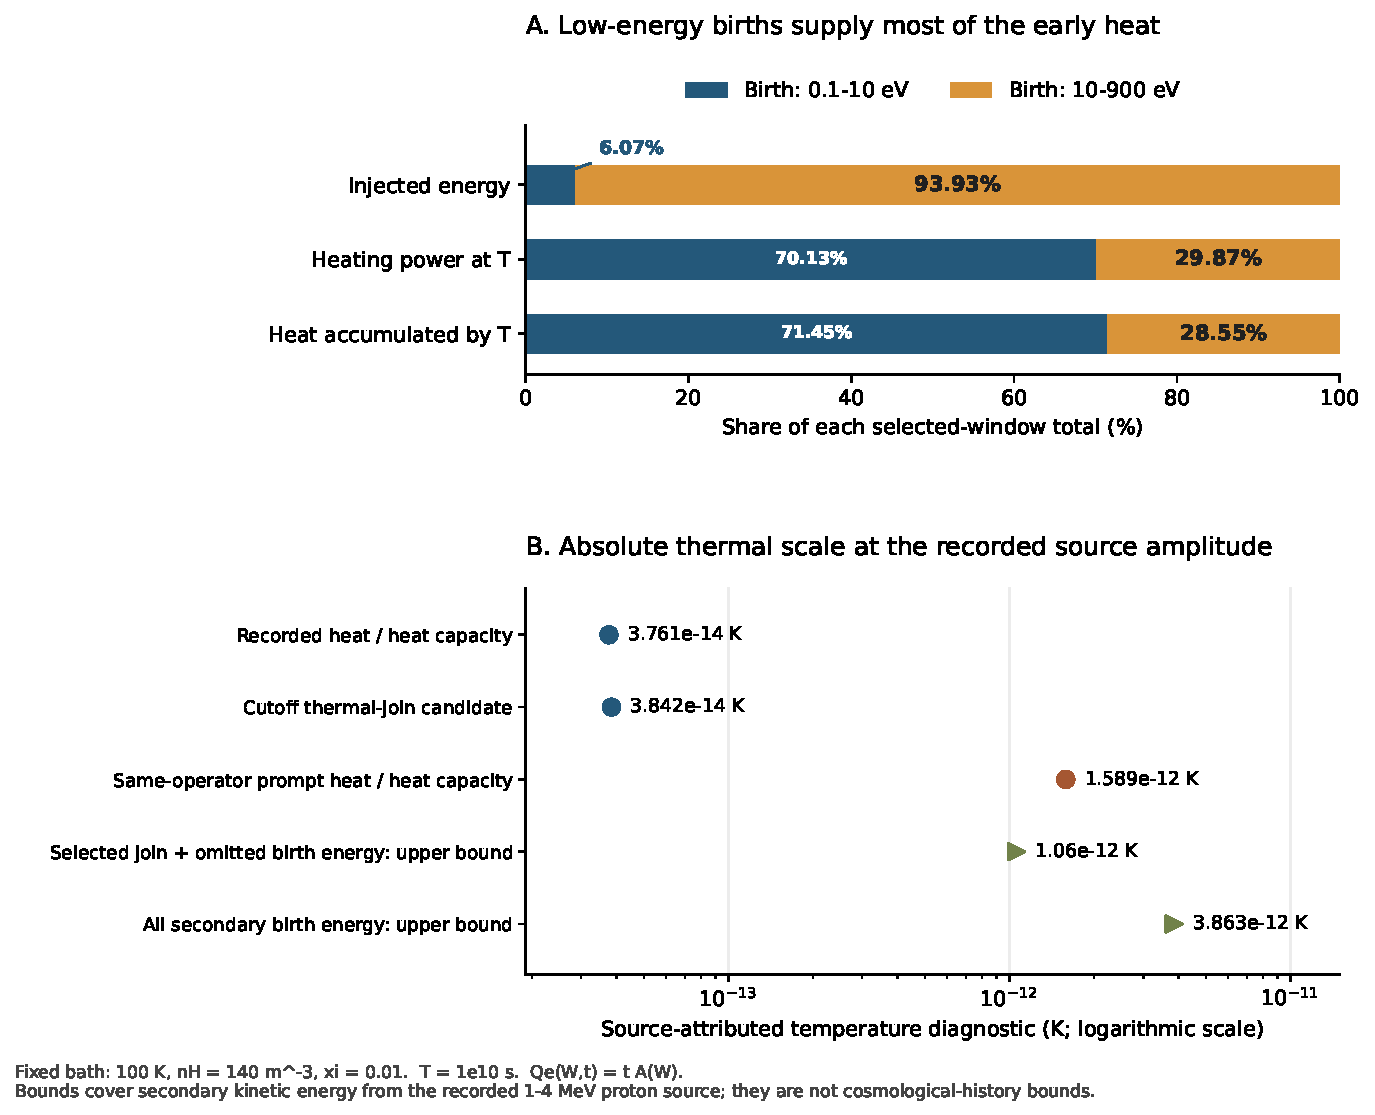
\includegraphics[width=\linewidth]{../results/SOURCE_BINDING_SUMMARY.pdf}
\caption{실제 source의 birth별 가열 기여와 절대 온도 척도. 위는 서로 다른 세 총량에 대한
birth 비율이며, 아래는 \(T_0\)에서의 계산값과 누적 상계를 구분한다. 새 시간 이력
곡선을 적분한 결과는 표시하지 않았다.}
\end{figure}

\section{검증, 독립 판정 및 근거의 경계}

계산 코드는 저장 소수를 Fraction으로 읽고 최종 값을 50자리 소수로 직렬화한다.
37개 확인에는 네 모형/표현 행의 과거 SI 출력 대조, birth별 출력과 합, source coverage,
zero source, energy ledger, number ledger 및 정확한 thermal energy algebra가 포함된다.
대조 허용오차 \(10^{-12}\)는 이번 기록 연결의 수치 기준이다. 실제 소비자 허용오차를
대신하지 않는다.\cite{calc}

첫 산술 실행에서는 zero-source 확인에 무차원 response fraction까지 합산하여 확인 한 개가
실패했다. source 진폭이 0이어도 무차원 \(H_0R\) 자체는 0이 될 필요가 없다.
dimensional energy/power만 검사하도록 수정했고 원 코드·결과·로그를 보존했다.
그 뒤 active/thermal 구분을 명시한 A2 계약으로 확장해 최종 실행을 마쳤다.
원 transport는 재실행하지 않았다.

독립 검토자의 최종 판정은 \texttt{PROMOTE\_SCOPED}이다. 후보 구현을 호출하지 않은 별도 기준 계산은 30개 PASS, 0개 실패, 종료 코드 0를 기록했다. 실제 입력·코드·결과의 읽기 범위, 독립 실행 및 적용 조건은 \path{review/DECISION.json}과 \path{review/REVIEW_KO.md}에 보존한다. 승격 대상은 실제 source에 결속한 고정 배경 응답, 명시한 cutoff 열적 편입 및 누적 에너지 예산이다. 전체 REI 채택과 cutoff 물리의 정밀도는 이 판정의 범위 밖이다.


\begin{itemize}[leftmargin=1.5em,itemsep=2pt]
\item source 단위·정규화·convolution 및 thermal accounting 식: 명시한 가정 아래 유도.
\item SI 값과 birth 비율: 저장된 원 실행값의 정확 산술 연결 및 기존 출력 대조.
\item outside-energy 상계: 기록된 birth energy를 조건으로 하는 수동적 에너지 예산.
\item 원자율·source window·leading local source의 물리 정확도: 상속한 근거 수준 유지.
\item cutoff 독립성 및 실제 REI 온도·이온화·광학깊이 history: 이후 채택 범위.
\end{itemize}

\section{DAG 개정과 다음 연구 단위}

국소 DAG에서 실제 BASS\_CR source binding을 완료로 분리하고 새 cutoff 편입 및 열적 관련성
결과를 그 범위에서 기록했다. 전역 RUX 노드 19개의 기존 상태와 의존관계는 유지한다.

\begin{center}
\begin{tabular}{P{.26\linewidth}P{.63\linewidth}}
\toprule
다음 작업 & 실제 입력과 완료 조건\\
\midrule
선택 이력 결속 & source 구간·진폭·시간 원점·초기 stock·bath가 이번 kernel 또는 그 변형 중
무엇을 필요로 하는지 한 실제 scenario에 명시한다.\\
Thermal 입자수 계약 & 총 자유전자, active 비열적 전자, thermal 전자를 구분하고 cutoff energy와
number의 이관 소유자를 정한다. 현재 원장을 재사용한다.\\
관측량 오차 예산 & 실제 observable, 양의 reference denominator, 절대 또는 상대 tolerance를
지정하고 이번 SI 가열·편입 항을 비교한다.\\
필요한 범위만 확장 & 선택 이력이 요구하는 누락 에너지·bath·시간·채널이 확인되면 해당 부족에
맞춘 다음 과학 계약을 만든다.\\
\bottomrule
\end{tabular}
\end{center}

현재 REI native pin은 FS10 terminal snapshot을 검사하는 인터페이스다.
새 causal source를 자동으로 받아들이는 인터페이스로 바꾸지 않았다.
\(\xi=0.1\) knot도 현재 \(\xi=0.01\) kernel의 확대 근거가 아니다.
국소 CR OFF 분기는 기존 구현과 근거를 재사용한다.

H 전체9600 추가 실행은 선택적 후속이고, F의 operator-binding 보류는 해당 경로에 남는다.
이번 source binding과 cutoff accounting은 그 경로의 자동 재시작을 요구하지 않는다.
다음 루프는 실제 source/입자수/허용오차를 연결하거나 명시된 독립 CR 질문으로 범위를 좁혀
진행할 수 있다.

\section{재현과 파일 안내}

\texttt{evaluate\_source\_binding.py}는 Python 표준 라이브러리만으로 실행된다.
입력 JSON, exact source manifest, 관련 원문, 첫 실패와 수정 기록, 최종 실행 로그, 독립 검토,
계획과 DAG를 함께 제공한다. 보고서와 그림은 결과 JSON에서 별도로 만든다.
\begin{verbatim}
python evaluate_source_binding.py
python render_results.py
python build_report_values.py
cd latex
xelatex -interaction=nonstopmode -halt-on-error report.tex
xelatex -interaction=nonstopmode -halt-on-error report.tex
\end{verbatim}
LaTeX source bundle은 Noto Sans CJK KR font와 라이선스를 포함한다.
전체 과거 H payload나 generator archive의 복제본이 아니라, 이번 scalar postprocess와
원문 계보를 재현하는 범위의 전달물이다.

\begin{thebibliography}{9}
\small
\bibitem{m0} 기존 M0 및 M1--M3의 \texttt{CACHED\_RESPONSE.json}.
출발 commit \texttt{4ca5a90de79c8fb82a25fd9e83615bec0dfa870b}.
이번 단위 \path{inputs/CACHED_RESPONSE.json}.
\bibitem{pulse} CR-PHYS02E 실제 pulse 반환 및 독립 범위 판정.
\path{inputs/PULSE_RECORD.json}, \path{inputs/PULSE_DECISION.json}.
\bibitem{paired} CR-PHYS02C paired9600 실제 결과 및 독립 closeout.
\path{inputs/PAIRED_RECORD.json}, \path{inputs/PAIRED_DECISION.json}.
\bibitem{source} 실제 source 호출 계보와 40개 source 읽기 기록.
\path{inputs/source_lineage/SOURCE_FINDINGS_KO.md},
\path{inputs/math_intake/SOURCE_INVENTORY.json}.
원문의 commit, 경로, Git blob, SHA256 및 읽은 범위를 보존한다.
\bibitem{coverage} PHYS02B source coverage.
\path{inputs/SOURCE_COVERAGE_RECORD.json}.
동일 constructor와 mesh 독립 적분 근거는 source lineage에 있다.
\bibitem{intake} 최신 BASS\_CR 및 REI 범위별 조사.
\path{inputs/CURRENT_BASS_CR_INTAKE.json},
\path{inputs/consumer_intake/SOURCE_IDENTITY.json}.
\bibitem{therm} 이번 cutoff energy/number 편입 유도.
\path{DERIVATION_KO.md}, \path{CONTRACT.json}의 A2.
\bibitem{calc} 실제 산술 출력과 원장 대조.
\path{results/SOURCE_BOUND_RESPONSE.json},
\path{evidence/POSTPROCESS_ACTUAL_EXECUTION.json},
\path{review/DECISION.json}.
\bibitem{md14} P. Madau and M. Dickinson, “Cosmic Star-Formation History,”
Annual Review of Astronomy and Astrophysics \textbf{52}, 415--486 (2014).
\href{https://arxiv.org/abs/1403.0007}{arXiv:1403.0007},
\href{https://doi.org/10.1146/annurev-astro-081811-125615}{doi:10.1146/annurev-astro-081811-125615}.
\end{thebibliography}
\end{document}
